\chapter{Experimental Evaluation\label{cha:chapter4}}

In this chapter we present findings that support the four ceilings, the negative-composability, the pre-flight ceiling-identification methodology and dispatch policy introduced in Chapter~\ref{cha:chapter3}.

The chapter is organised around the ceilings rather than around individual ablations, meaning that a Cargo feature can be positive evidence for one ceiling and null evidence for another.

The chapter is structured as follows:

\begin{table}[H]
  \centering
  \caption{Chapter roadmap.}
  \label{tab:exp:roadmap}
  \begin{tabular}{ll}
    \toprule
    Section & Content \\
    \midrule
    §\ref{sec:exp:python} & Scale of the Python baseline \\
    §\ref{sec:exp:guide} & Reading guide to the four-ceiling structure \\
    §\ref{sec:exp:c1}--§\ref{sec:exp:c4} & Evidence and mechanism for each ceiling \\
    §\ref{sec:exp:scaling} & Multi-core scaling and SMT contention \\
    §\ref{sec:exp:wf} & Work-fragmentation regime (columnar, query-batch, morsel) \\
    §\ref{sec:exp:negcomp} & Negative-composability pattern and pre-flight methodology \\
    §\ref{sec:exp:reindex} & Per-cluster reindexing falsification \\
    §\ref{sec:exp:dispatch} & Dispatch policy and in-distribution validation \\
    §\ref{sec:exp:ood} & Out-of-distribution validation \\
    §\ref{sec:exp:e2e} & End-to-end comparison against the Python baseline \\
    §\ref{sec:exp:rebinning} & Rust rebinning kernel \\
    §\ref{sec:exp:variance} & Variance check on borderline claims \\
    §\ref{sec:exp:summary} & Summary: hypotheses and verdicts \\
    \bottomrule
  \end{tabular}
\end{table}

Hardware, software, datasets, and the measurement protocol are documented in Chapter~\ref{cha:chapter3} and are not restated here.

\section{Python Baseline\label{sec:exp:python}}

The Python baseline (\texttt{FAINDER\_NO\_RUST=1}) is the unmodified Fainder library running under \texttt{with-results}.

\subsection{Wall-Clock at Three Scales\label{sec:exp:python:wall}}

\begin{table}[H]
  \centering
  \caption{Python baseline wall-clock, median of 5 reps, \texttt{with-results} mode, 10K queries. The \texttt{c256\_56gb} cell exceeds the per-run cap; its wall is measured via a 1K-query subsample scaled $\times 10$ (§\ref{sec:exp:e2e:mat}).}
  \label{tab:python_wall}
  \begin{tabular}{lrrrrrr}
    \toprule
    Dataset & $t{=}1$ & $t{=}8$ & $t{=}16$ & $t{=}32$ & $t{=}64$ & $t{=}96$ \\
    \midrule
    \texttt{c256\_10gb} & $610.2$\,s & $601.5$\,s & $599.7$\,s & $596.3$\,s & $600.2$\,s & $601.6$\,s \\
    \texttt{c256\_30gb} & -- & -- & $1\,890.3$\,s & -- & -- & -- \\
    \texttt{c256\_56gb} & -- & -- & $8\,589$\,s & -- & -- & -- \\
    \bottomrule
  \end{tabular}
\end{table}

On the production server, we observe run-to-run variance of $\pm 3$--$6\%$ at $t=16$ and $\pm 5$--$12\%$ at $t \in \{32, 64\}$. We use this variance band for the remainder of the thesis: effects below $\pm 8\%$ in single-run tables are described as ``within noise''.

Two observations for the Python baseline:

\begin{enumerate}
  \item Python's wall clock is \emph{flat} across all thread counts on \texttt{c256\_10gb} with a $2\%$ spread. This is due to the GIL: \texttt{numpy.searchsorted} does not release it, so \texttt{FAINDER\_NUM\_THREADS} is silently ignored. Threading buys nothing in Python.
  \item Python's IPC at $t{=}16$ is \emph{higher} than the Rust default engine's ($2.35$ vs $0.96$, with-results on both), yet its wall is $378\times$ longer on the same cell. NumPy's bulk operations on contiguous arrays are cache-friendly and pipeline well, but the GIL serialises the whole run onto one effective core, and Python retires $6.2\times$ the instructions on per-\emph{(query, cluster)} bookkeeping and result materialisation (§\ref{sec:exp:e2e:mat}).
\end{enumerate}

 The Rust engine wins by executing fewer instructions across all cores in parallel, not by winning on IPC.

\section{Reading Guide: The Four Ceilings\label{sec:exp:guide}}

Before getting into specific ablations, we note that the ceiling for Fainder's percentile queries on this hardware is \emph{never} ceiling~(i). Every latency-side ablation measures null within noise, the mechanism and per-cell numbers live in §\ref{sec:exp:c1}. The reading guide below points each of ceilings (ii)--(iv) at the section where its evidence lands.

The four ceilings are, in order of increasing thread count:

\begin{enumerate}
  \item \textbf{Ceiling (i): Single-thread compute / L1 latency.} Does \emph{not} bind on our workload for this hardware.
  \item \textbf{Ceiling (ii): Shared L3 capacity.} At low and moderate thread counts on the larger datasets, the per-thread working set sums above the L3 capacity and binds.
  \item \textbf{Ceiling (iii): On-socket memory-traffic pressure.} At high thread counts on the largest dataset, an anti-scaling wall-time signature appears.
  \item \textbf{Ceiling (iv): Cross-socket UPI interconnect.} Spans both sockets at $t > 48$.
\end{enumerate}

We also observe two further regimes (HT-sibling contention and work-fragmentation) that recur across the ceilings. \emph{HT-sibling contention} occurs at $t > 96$ and is addressed in §\ref{sec:exp:scaling}. \emph{Work-fragmentation} occurs at high $t$ on big data, and is addressed in §\ref{sec:exp:wf}.

\begin{figure}[H]
  \centering
  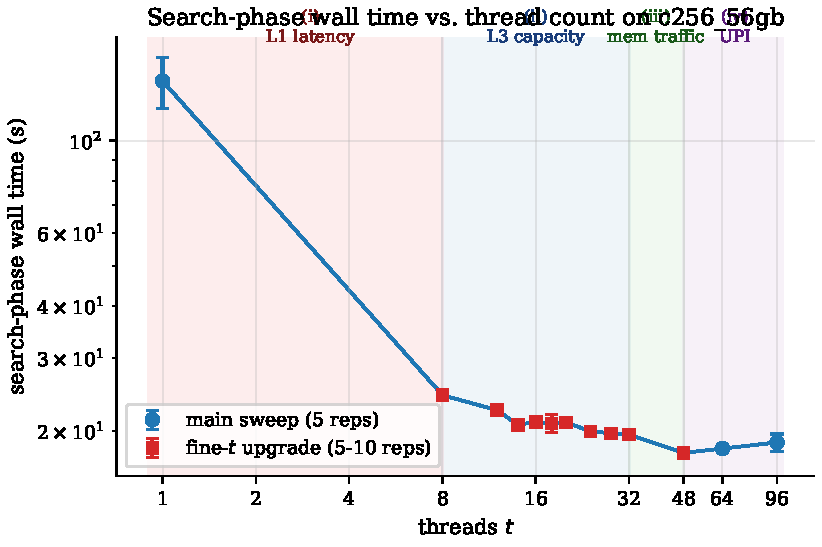
\includegraphics[width=0.9\linewidth]{img/gen/ch4_four_ceilings.pdf}
  \caption{Search-phase wall time of the default (SoA + f32) build on \texttt{c256\_56gb} across thread counts. Both axes are log-scaled. Shaded areas signify the regimes in which each ceiling binds: (i) single-thread compute / L1 latency at $t \leq 8$, (ii) shared L3 capacity at $t \in [8, 32]$, (iii) on-socket memory-traffic pressure at $t \in [32, 48]$, and (iv) cross-socket UPI interconnect at $t > 48$. Error bars show $95\%$ CIs from the 5-repetition measurements.}
  \label{fig:exp:four_ceilings}
\end{figure}

\section{Ceiling (i): Single-Thread Compute / L1 Latency\label{sec:exp:c1}}

Ceiling (i) is best tested in the single-thread regime, since there are no inter-thread effects to skew the measurement. We perform four ablation experiments addressing this ceiling from different angles: 
\begin{enumerate}
  \item AVX-512 leaf-stage SIMD (§\ref{sec:exp:c1:simd})
  \item 8-way pipelined batch-search (§\ref{sec:exp:c1:batch})
  \item 16-query horizontal-SIMD lockstep (§\ref{sec:exp:c1:horizontal})
  \item PGM learned-index (§\ref{sec:exp:c1:pgm})
\end{enumerate}

The results are null or marginal. A fifth latency-side variant, 4-way branchless k-ary search, was evaluated in an earlier campaign and dropped from the final build.

\paragraph{The Dependent-Load Chain in \texttt{partition\_point}.}

The hot loop per-cluster is the two binary searches in \texttt{partition\_point} (§\ref{sec:bg:partition_point}). The first search is over the bin-boundary array, the second is over the column slice of the cluster. The size of the bin-boundary array is fixed at ${\sim}142$; the size of the column slice is $n_\text{hists}$. The first fits into two L1d cache lines, the second fits into L2 but exceeds L1d on the larger datasets. Each iteration of each search is a dependent load that must wait for the previous iteration to complete. This dependent load chain \emph{is} the wall time per cluster on this workload.

\subsection{Ablation A: AVX-512 Leaf-Stage SIMD\label{sec:exp:c1:simd}}

The \texttt{simd} feature replaces the last ${\sim}16$ elements of \texttt{partition\_point} with one AVX-512 vector compare. This does not alter the dependent-load chain above the leaf, but it removes the last ${\sim}16$ dependent loads from the chain, shaving one iteration's latency from the inner loop.

\begin{table}[H]
  \centering
  \caption{\texttt{simd} vs default, suppress mode, median of 5. Ratio $<$ 1 means \texttt{simd} faster.}
  \label{tab:simd}
  \begin{tabular}{lrrrrrr}
    \toprule
    Dataset & $t{=}1$ & $t{=}8$ & $t{=}16$ & $t{=}32$ & $t{=}64$ & $t{=}96$ \\
    \midrule
    \texttt{c256\_10gb} & $1.04\times$ & $1.00\times$ & $0.98\times$ & $1.03\times$ & $0.97\times$ & $0.93\times$ \\
    \texttt{c256\_30gb} & $1.03\times$ & $1.01\times$ & $1.02\times$ & $1.00\times$ & $0.90\times$ & $0.95\times$ \\
    \texttt{c256\_56gb} & $1.07\times$ & $0.93\times$ & $1.04\times$ & $0.94\times$ & $0.96\times$ & $0.99\times$ \\
    \bottomrule
  \end{tabular}
\end{table}

The range of $0.90$--$1.07\times$ is within run-to-run noise across all 18 cells. \emph{SIMD} is not a ceiling-(i) win. The leaf vectoriser's job (removing the last ${\sim}16$ dependent loads) is correct, but it does not address the part of the dependency chain, that is the bottleneck. 

\subsection{Ablation B: 8-Way Batch-Search\label{sec:exp:c1:batch}}

\texttt{batch-search} is a columnar-only feature (mutually exclusive with \texttt{horizontal-\allowbreak simd}) that pipelines eight binary searches through the CPU's MSHR (Miss Status Holding Register) budget, sharing early-stage midpoint loads. Since queries are grouped by bin index $k^*$, it is only meaningful inside the column-centric engine. We compare to the columnar default.

\begin{table}[H]
  \centering
  \caption{\texttt{batch-search} vs \texttt{columnar-default}, suppress mode, median of 5. Ratio $<$ 1 means \texttt{batch-search} faster.}
  \label{tab:batchsearch}
  \begin{tabular}{lrrrrrr}
    \toprule
    Dataset & $t{=}1$ & $t{=}8$ & $t{=}16$ & $t{=}32$ & $t{=}64$ & $t{=}96$ \\
    \midrule
    \texttt{c256\_10gb} & $0.98\times$ & $1.05\times$ & $1.02\times$ & $1.00\times$ & $0.97\times$ & $1.01\times$ \\
    \texttt{c256\_30gb} & $1.09\times$ & $1.05\times$ & $1.05\times$ & $0.98\times$ & $1.00\times$ & $1.00\times$ \\
    \texttt{c256\_56gb} & $0.99\times$ & $1.01\times$ & $0.96\times$ & $0.99\times$ & $1.01\times$ & $0.99\times$ \\
    \bottomrule
  \end{tabular}
\end{table}

Across all 18 cells, the range is $0.96$--$1.09\times$, indistinguishable from noise, for the main workload \emph{c256\_56gb} the range is even tighter at $\pm 4\%$. 

This does not mean that \texttt{batch-search} is broken, the dependent-load chain above the leaf is not the bottleneck. The ceiling-(i) hypothesis is falsified.

\subsection{Ablation C: Horizontal-SIMD Lockstep\label{sec:exp:c1:horizontal}}

\texttt{horizontal-simd} \cite{polychroniou_2014} is columnar-only (mutually exclusive with \texttt{batch-search}). It vectorises 16 queries' bisection trees in tandem through one column, rather than within a single query. Structurally different from \texttt{simd}, but identical conclusion: the dependent-load chain above the leaf is not the bottleneck.

\begin{table}[H]
  \centering
  \caption{\texttt{horizontal-simd} vs \texttt{columnar-default}, suppress mode, median of 5. Ratio $<$ 1 means \texttt{horizontal-simd} faster.}
  \label{tab:horizsimd}
  \begin{tabular}{lrrrrrr}
    \toprule
    Dataset & $t{=}1$ & $t{=}8$ & $t{=}16$ & $t{=}32$ & $t{=}64$ & $t{=}96$ \\
    \midrule
    \texttt{c256\_10gb} & $0.95\times$ & $1.03\times$ & $1.06\times$ & $1.05\times$ & $0.96\times$ & $1.00\times$ \\
    \texttt{c256\_30gb} & $1.07\times$ & $1.06\times$ & $1.12\times$ & $1.03\times$ & $0.95\times$ & $1.00\times$ \\
    \texttt{c256\_56gb} & $1.02\times$ & $1.00\times$ & $0.99\times$ & $1.01\times$ & $0.98\times$ & $1.00\times$ \\
    \bottomrule
  \end{tabular}
\end{table}

Across all 18 cells, the range is $0.95$--$1.12\times$, which fits within the run-to-run noise. It does show a mild regression signature at intermediate $t$ on \texttt{c256\_30gb} where the L3-capacity ceiling begins to bind (§\ref{sec:exp:c2}). 

\subsection{Ablation D: PGM Learned Index\label{sec:exp:c1:pgm}}

\texttt{pgm} replaces binary-search with a learned-index segment lookup plus a small scan. The mechanism is described in §\ref{sec:method:impl:variants}. It was tested in all engines (row-centric, column-centric, query-batch) and the measurement here uses the row-centric default.

The dependent loads per cluster drop to $O(\log \log n)$ (Since the PGM segment lookup is near constant time) as intended, but wall does not move because wall was not bounded by those cycles to begin with. If ceiling~(i) bound, this would be the most direct attack possible.

\begin{table}[H]
  \centering
  \caption{\texttt{pgm} vs \texttt{default} (row-centric), suppress mode, median of 5. Ratio $<$ 1 means \texttt{pgm} faster.}
  \label{tab:pgm}
  \begin{tabular}{lrrrrrr}
    \toprule
    Dataset & $t{=}1$ & $t{=}8$ & $t{=}16$ & $t{=}32$ & $t{=}64$ & $t{=}96$ \\
    \midrule
    \texttt{c256\_10gb} & $1.12\times$ & $1.02\times$ & $1.00\times$ & $1.03\times$ & $1.05\times$ & $0.92\times$ \\
    \texttt{c256\_30gb} & $1.02\times$ & $1.13\times$ & $0.96\times$ & $1.05\times$ & $1.12\times$ & $0.92\times$ \\
    \texttt{c256\_56gb} & $0.91\times$ & $1.10\times$ & $1.00\times$ & $0.95\times$ & $0.99\times$ & $0.97\times$ \\
    \bottomrule
  \end{tabular}
\end{table}

Across all $18$ cells, the range is $0.91$--$1.13\times$. No single cell is an unambiguous win. Our largest win ($-9\%$ at \texttt{c256\_56gb} $t=1$) is matched by a similar-sized loss ($+13\%$ at \texttt{c256\_30gb} $t=8$). Perf counters confirm the $\log_2 n$ dependent-load cycles per cluster drop to $O(\log \log n)$ as intended, but since the dependent-load chain was not the bottleneck, wall does not move.

\subsection{Mechanism Evidence\label{sec:exp:c1:mechanism}}

Hot-loop counters Per-cluster on the default build (single thread) show the dependent-load chain dominates cycle budget. IPC is $1.80$ on \texttt{c256\_10gb}, $1.93$ on \texttt{c256\_30gb}, $1.87$ on \texttt{c256\_56gb}, all comfortably below the retirement ceiling and points to a load-latency-bound loop. The L1d miss-per-load rate at $t{=}1$ is $\sim\!0.49$--$0.68\%$ across the three datasets. Neither the misprediction rate nor the L1d-miss rate exceed the noise floor that the ablations were designed to reduce.

This resolves the apparent tension with the chain being the wall time: the binding quantity is the \emph{number} of dependent chains, one per cluster, not the depth or throughput of any single chain (which scales only as $\log_2$ of the bins per cluster). The four ablations shorten or pipeline individual chains; none of them reduces the count. That is why they all measure null.

Ceiling~(i) is part of the ceiling taxonomy due to it being the most commonly assumed default ceiling in the published literature on in-memory percentile and binary-search workloads. Kim et al.'s FAST index~\cite{kim_2010} explicitly co-optimises for cache-line, page, and SIMD width on the assumption that L1-latency and CMOV-chain length bind search cost, Khuong and Morin~\cite{khuong_morin_2017} benchmark array layouts under the same assumption, Ferragina and Vinciguerra's PGM~\cite{ferragina_2020} addresses the $\log_2 n$ dependent-load chain as its whole motivation, and Schlegel et al.'s SIMD $k$-ary search~\cite{schlegel_2009} treats the same chain as the cost to be shortened.

Our falsification of ceiling~(i) is what gives credit to the other ceilings and gives us the opportunity to set aside the single-thread compute assumption and reason about the other ceilings. This negative result is positive evidence about binding constraints.

\section{Ceiling (ii): Shared L3 Capacity\label{sec:exp:c2}}

The aggregate per-thread working set sums above the L3 shared capacity of $105$\,MiB per socket at moderate thread counts on the \emph{larger} datasets. We observe a thread-scaling curve that shows a bend before saturating the cores. Optimisations that shrink the per-thread footprint should improve this ceiling; optimisations that expand it should worsen it. The mechanism reading (§\ref{sec:exp:c2:mechanism}) refines this picture: what binds at moderate $t$ is regime-dependent, allocator-arena contention on dense clusters and aggregate L3 footprint at the sparser OOD density.

\subsection{SoA vs AoS\label{sec:exp:c2:soa}}

The default uses SoA. The \texttt{aos} feature is the negative control: every cache line loaded during the search now also carries an unused 32-bit ID field, halving the useful values per line.

\begin{table}[H]
  \centering
  \caption{\texttt{aos} vs default, suppress mode, median of 5 reps. Ratio $>$ 1 means \texttt{aos} slower; ratio $<$ 1 means \texttt{aos} \emph{faster} (bold cells).}
  \label{tab:aos}
  \begin{tabular}{lrrrrrr}
    \toprule
    Dataset & $t{=}1$ & $t{=}8$ & $t{=}16$ & $t{=}32$ & $t{=}64$ & $t{=}96$ \\
    \midrule
    \texttt{c256\_10gb} & $1.11\times$ & $1.05\times$ & $1.03\times$ & $\mathbf{0.98\times}$ & $1.07\times$ & $1.09\times$ \\
    \texttt{c256\_30gb} & $1.09\times$ & $1.07\times$ & $1.04\times$ & $1.06\times$ & $1.12\times$ & $\mathbf{0.94\times}$ \\
    \texttt{c256\_56gb} & $1.03\times$ & $1.17\times$ & $1.02\times$ & $1.00\times$ & $\mathbf{0.96\times}$ & $\mathbf{0.99\times}$ \\
    \bottomrule
  \end{tabular}
\end{table}

The primary workload \texttt{c256\_56gb} observes a $+17\%$ penalty at $t=8$ in the L3-capacity regime, but then flips to a small $-4\%$ gain at $t=64$. We do not consider this flip run-to-run noise, but an indicator of a ceiling-(ii)$\to$ceiling-(iii) transition of the binding constraint. AoS is negatively impacted  by the doubled per-line footprint in the L3-capacity regime, as confirmed by an $\sim\!+0.05$\, L1d-miss-per-instruction increase at $t=8$ versus SoA and the roughly doubled per-socket L3 working set at $t \in [8, 32]$.

AoS no longer becomes the binding cost, once on-socket memory-traffic pressure binds at $t \ge 48$, since the higher spatial locality of the interleaved (AoS) layout on the ID emit leaves a bit of room for improvement. We observe this also on \texttt{c256\_30gb} (t=96 flips to $-6\%$) but not on \texttt{c256\_10gb}, since its working set stays L2-resident, ceiling~(ii) never binds. SoA continues to be the right default for the composed bundle at $t=16$ where the wall budget matters most, but the layout choice is regime-conditional, rather than absolute.

Figure~\ref{fig:exp:aos_flip} shows the same measurement as a delta versus default across the finer thread sweep on \texttt{c256\_56gb}.

\begin{figure}[H]
  \centering
  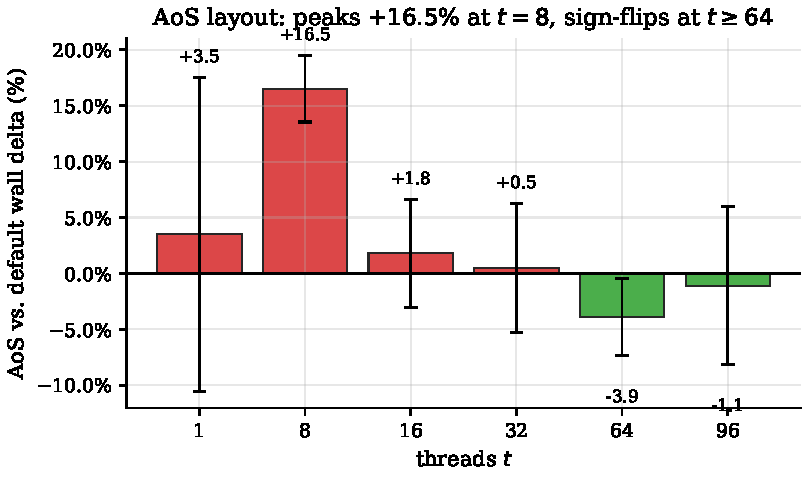
\includegraphics[width=0.9\linewidth]{img/gen/ch4_aos_flip.pdf}
  \caption{AoS layout wall-time delta versus default (SoA + f32) on \texttt{c256\_56gb} across threads. Red bars: AoS slower. Green bars: AoS faster. Error bars show $95\%$ CIs propagated through the delta computation.}
  \label{fig:exp:aos_flip}
\end{figure}

\subsection{f16 Footprint Halving\label{sec:exp:c2:f16}}

\texttt{f16} stores values as 16-bit half-precision floats that dequantise during comparison. We predict that \texttt{f16} wins in the regime where the f32 footprint exceeds L3 per socket but the f16 footprint fits, with the win largest at moderate $t$ on the larger datasets.

\begin{itemize}
  \item Standalone on \texttt{c256\_56gb}: no cell shows a statistically significant \texttt{f16} win. Figure~\ref{fig:exp:f16_finet} shows two significant losses at $t{=}8$ and $t{=}14$, every other cell in the $10$-rep fine-$t$ sweep straddles zero.
  \item Standalone on \texttt{c256\_30gb}: also no clear win. Deltas range from $-12\%$ (at $t{=}96$) to $+3.5\%$ (at $t{=}8$). The predicted L3-footprint win at $t{=}16$ ($+3.1\%$) is a small loss instead.
  \item Inside the bundled \bcombo{} build at $t{=}16$ on \texttt{c256\_56gb}, the bundle runs at $0.773\times$ default wall ($22.7\%$ speedup).
  \item \texttt{f16} isolation measures \texttt{f16}'s contribution to the bundle: we find a \emph{regime-dependent sign reversal} on the primary workload; \texttt{c256\_56gb} at $t{=}16$, \bcombo{} without \texttt{f16} at $13.54$\,s is $15.6\%$ \emph{faster} than \bcombo{} at $16.03$\,s meaning that \emph{f16} drags the net bundle down (and $-16.2\%$ at $t{=}32$, only at $t{=}64$ and $t{=}96$ does removing \texttt{f16} produce a small $\sim\!3\%$ cost). On the sparser OOD workload \texttt{c1024\_56gb} (§\ref{sec:exp:ood}) at the same $t{=}16$, removing \texttt{f16} costs $+20.9\%$, so \texttt{f16} saves $20.9\%$ inside the bundle.
  \item The reversal is \emph{density-dependent}. On \texttt{c256\_56gb} the per-cluster f32 slice ($\sim\!105$\,KiB) exceeds L1d and is L2-resident; halving it does not unlock a new cache-resident regime, while paying f16$\to$f32 conversion costs on every comparison. The mechanism is developed further in §\ref{sec:exp:c2:mechanism}.
  \item \texttt{f16} is a bundle drag that the other five features have to absorb. At the sparser OOD density, \texttt{f16} carries roughly a fifth of the bundle win.
\end{itemize}

\begin{figure}[H]
  \centering
  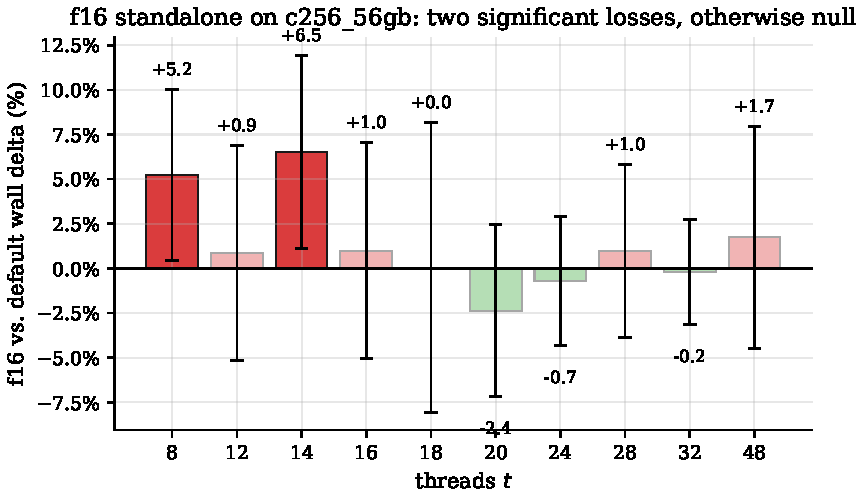
\includegraphics[width=0.9\linewidth]{img/gen/ch4_f16_finet.pdf}
  \caption{\texttt{f16} vs.\ default wall-time delta on \texttt{c256\_56gb}. Saturated bars mark cells where $t$ $95\%$ CI (dof $= n_a + n_b - 2$, §\ref{sec:method:ci}) excludes zero, pale bars are noise-band.}
  \label{fig:exp:f16_finet}
\end{figure}

 

\subsection{Pooled Output Buffer\label{sec:exp:c2:pooled}}

\texttt{pooled} is a bundle feature that pre-allocates the output buffer for each query, rather than allocating one per matching cluster. The intended mechanism is a smaller per-thread allocator footprint and elimination of the glibc arena mutex contention from §\ref{sec:exp:c2:mechanism}.

\begin{table}[H]
  \centering
  \caption{\texttt{pooled} vs default, suppress mode. Ratio $<1$ means \texttt{pooled} faster.}
  \label{tab:pooled}
  \begin{tabular}{lrrrrrr}
    \toprule
    Dataset & $t{=}1$ & $t{=}8$ & $t{=}16$ & $t{=}32$ & $t{=}64$ & $t{=}96$ \\
    \midrule
    \texttt{c256\_10gb} & $\mathbf{0.51\times}$ & $\mathbf{0.75\times}$ & $\mathbf{0.94\times}$ & $0.99\times$ & $1.03\times$ & $\mathbf{0.88\times}$ \\
    \texttt{c256\_30gb} & $\mathbf{0.57\times}$ & $\mathbf{0.73\times}$ & $1.00\times$ & $0.98\times$ & $1.07\times$ & $1.42\times$ \\
    \texttt{c256\_56gb} & $\mathbf{0.53\times}$ & $\mathbf{0.66\times}$ & $\mathbf{0.80\times}$ & $\mathbf{0.95\times}$ & $\mathbf{0.93\times}$ & $1.02\times$ \\
    \bottomrule
  \end{tabular}
\end{table}

Measurements confirm the arena-mutex mechanism at scale. On \texttt{c256\_56gb} \texttt{pooled} standalone wins $-46.9\%$ at $t{=}1$, $-34.1\%$ at $t{=}8$, and $-20.2\%$ at $t{=}16$. On the primary workload at $t{=}16$, \texttt{pooled} carries essentially the entire bundle win, with the other five features (including \texttt{f16}) providing a small net loss that \texttt{pooled}'s cushion absorbs.

The wins compress at higher $t$ on the two smaller datasets and even flip negative on \texttt{c256\_30gb} at $t{=}96$. At low $t$ the allocator arena mutex serialises threads on the shared glibc arena, at high $t$ other ceilings (memory-traffic pressure, UPI) dominate and the arena is no longer the binding cost, so \texttt{pooled}'s cushion has less to protect against.

\paragraph{Bundle-minus-pooled isolation}

The direct \bcombo{}-minus-\texttt{pooled} sweep on \texttt{c256\_56gb} reveals a shape as regime-dependent as the \texttt{f16} isolation of §\ref{sec:exp:c2:f16}:

\begin{table}[H]
  \centering
  \caption{\bcombo{}-minus-\texttt{pooled} vs full \bcombo{}. Positive removal cost means \texttt{pooled} was helping the bundle, negative means \texttt{pooled} was \emph{hurting} it.}
  \label{tab:pooled_isolation}
  \footnotesize
  \begin{tabular}{lrrrrrr}
    \toprule
    & $t{=}1$ & $t{=}8$ & $t{=}16$ & $t{=}32$ & $t{=}64$ & $t{=}96$ \\
    \midrule
    \bcombo{} wall (s)          & $117.6$ & $18.9$ & $16.0$ & $16.6$ & $19.1$ & $20.5$ \\
    \texttt{bs}-minus-\texttt{pooled} wall (s) & $181.9$ & $26.0$ & $16.7$ & $15.1$ & $18.5$ & $20.9$ \\
    \texttt{pooled} bundle contribution & $+54.7\%$ & $+37.1\%$ & $+4.4\%$ & $\mathbf{-9.4\%}$ & $\mathbf{-3.2\%}$ & $+1.8\%$ \\
    \bottomrule
  \end{tabular}
\end{table}

This is a second inside-bundle sign-flip alongside \texttt{f16}'s (§\ref{sec:exp:c2:f16}): an optimisation that decisively wins standalone can turn into a bundle drag at a different regime cell. The direction of the drag is set by which ceiling binds at the composition. §\ref{sec:exp:c2:mechanism} dives deeper into the two-feature reversal mechanism.

\subsection{Mechanism Reading\label{sec:exp:c2:mechanism}}

Ceiling~(ii) binds at moderate $t$ on the larger datasets. Although, this binding is less straightforward than pure L3 capacity. It is regime-dependent like the direct standalone and bundle-isolation measurements now let us name.

The first binding constraint on the  primary workload at moderate $t$ is allocator-arena mutex contention instead of L3 capacity. \texttt{pooled}'s job was to address the mutex by removing per-cluster vector allocation, which it wins $-20.2\%$ at $t{=}16$. After that, the two direct bundle isolations show that neither \texttt{f16} nor \texttt{pooled} compose cleanly.

\begin{itemize}
  \item \texttt{f16} standalone wins nothing at any $t$ on \texttt{c256\_56gb}, and inside the bundle it is a $+15.6\%$ drag at $t{=}16$: removing \texttt{f16} makes the bundle faster.
  \item \texttt{pooled} standalone wins $-20.2\%$ at $t{=}16$, but inside the bundle its contribution collapses to $+4.4\%$ at $t{=}16$ and \emph{flips sign} at $t{=}32$--$64$, where removing \texttt{pooled} makes the bundle $-9.4\%$/$-3.2\%$ faster.
\end{itemize}

As formalised in §\ref{sec:exp:negcomp}, the ceiling that binds at a given regime cell is not necessarily the same ceiling that bound at a different regime cell. The ceiling that binds at $t{=}16$ is allocator-arena mutex contention, which \texttt{pooled} addresses. The ceiling that binds at $t{=}32$--$64$ is on-socket memory-traffic pressure, which \texttt{pooled} does not address and whose contention costs it adds to.

For the OOD workload \texttt{c1024\_56gb}, we observe a different ceiling-(ii) mechanism. A per-cluster f32 slice ($\sim\!33$\,KiB) fits in L1d, but the $610$ effective clusters (vs.\ $191$ on \texttt{c256\_56gb}) mean the aggregate cluster-loop working set is proportionally larger. \texttt{f16}'s halving pays back by $\sim\!20\%$ inside the bundle. Ceiling (ii) thus covers arena-mutex serialisation on dense clusters, L3-aggregate footprint pressure on sparse many-clusters, showing that the ceiling is not a single mechanism but a regime-dependent set of mechanisms. We can separate the two with our standalone-vs-bundle sign-flip on \texttt{f16} between the two workloads, which is the empirical evidence that they are separate.

Two mechanistic details to note:

\begin{itemize}
  \item \texttt{mimalloc} standalone \emph{hurts} at low-$t$ on \texttt{c256\_56gb} (+22\% at $t{=}1$ and $t{=}8$) but wins $-10\%$ at $t{=}32$. The regression at lower thread counts is likely due to mimalloc's per-thread arena warmup dominating.
  \item \texttt{pin-cores} standalone wins $-19\%$ at $t{=}32$ and is neutral to mildly negative at $t{=}64$--$96$. $t \geq 64$ is already contended by SMT threads on the same physical core, so \texttt{pin-cores} cannot help. 
\end{itemize}

We don't consider either \texttt{mimalloc} or \texttt{pin-cores} to be a ceiling-(ii) win in isolation, but they are both useful inside the bundle at their own regime cells.

\section{Ceiling (iii): On-Socket Memory-Traffic Pressure\label{sec:exp:c3}}

At high $t$ on the larger datasets, the DDR5 per-socket bandwidth budget (${\sim}300$\,GB/s) saturates. We observe \emph{anti-scaling}: wall-clock rises while cores are added past the saturation point. Optimisations that could improve this ceiling include reducing bytes-per-emit or bytes-per-comparison.

\paragraph{Anti-Scaling Signature.}\label{sec:exp:c3:anti}

Adding more cores does not add more bandwidth past the channel limit, and the cross-thread contention costs grow.

At \texttt{c256\_30gb} $t{=}96$, the default build takes $5.89$\,s, which is $+42\%$ slower than $t{=}64$ at $4.14$\,s.

Perf counters at $t=96$ on default \texttt{c256\_30gb}: IPC drops to $0.55$ from $1.93$ at $t=1$, and the LLC-miss count rises by $1.6\times$ between $t=64$ and $t=96$. The same dataset under \texttt{packed-ids} only goes $3.88$\,s $\rightarrow$ $4.70$\,s, a $+21\%$ slowdown over the same $t$ step.

\subsection{\texttt{packed-ids}: Bit-Packed Emit Phase\label{sec:exp:c3:packed}}

The \texttt{packed-ids} feature compresses the emit-phase ID bandwidth from $32$ bits per ID to ${\sim}20$ bits (the actual maximum global ID in the cluster). The decoder is $\sim\!3$ instructions per ID, the bandwidth saving is ${\sim}37\%$ on \texttt{c256\_10gb}.

\begin{table}[H]
  \centering
  \caption{\texttt{packed-ids} vs default, suppress mode, median of 5. Ratio $<$ 1 means \texttt{packed-ids} faster.}
  \label{tab:packed}
  \begin{tabular}{lrrrrrr}
    \toprule
    Dataset & $t{=}1$ & $t{=}8$ & $t{=}16$ & $t{=}32$ & $t{=}64$ & $t{=}96$ \\
    \midrule
    \texttt{c256\_10gb} & $0.94\times$ & $0.91\times$ & $1.00\times$ & $0.94\times$ & $1.04\times$ & $0.92\times$ \\
    \texttt{c256\_30gb} & $0.92\times$ & $0.86\times$ & $0.91\times$ & $0.95\times$ & $0.94\times$ & $\mathbf{0.80\times}$ \\
    \texttt{c256\_56gb} & $\mathbf{0.83\times}$ & $0.97\times$ & $0.96\times$ & $0.98\times$ & $0.91\times$ & $0.97\times$ \\
    \bottomrule
  \end{tabular}
\end{table}

Range $0.80$--$1.04\times$. Three cells show the largest wins with different mechanisms:

\begin{itemize}
  \item \textbf{30gb $t{=}96$ ($-20\%$).} bandwidth-saturation case. Default scales anti-monotonically ($t{=}64 \rightarrow t{=}96$: $4.15$\,s $\rightarrow$ $5.89$\,s), \texttt{packed-ids} is effective here since it reduces per-id bandwidth.
  \item \textbf{56gb $t{=}1$ ($-17\%$).} L3-capacity pressure at low $t$. The 56\,GB index footprint exceeds the $105$\,MiB shared LLC per socket even with one thread holding it. Reading $20$ bits/id instead of $32$ reduces capacity-miss rate, so each id costs fewer DRAM round-trips.
  \item \textbf{56gb $t{=}64$ ($-9\%$).} Bandwidth before HT-contention dominates, the saving partially translates into a wall win.
\end{itemize}

Once again, the win pattern follows regimes instead of mechanisms, which is why a ceiling-organised framing is useful.

\paragraph{\texttt{mimalloc}: Allocator Sub-Ceiling.}\label{sec:exp:c3:mimalloc}

\texttt{mimalloc} is a drop-in replacement for glibc malloc. It uses per-thread sharded free lists to reduce allocator contention. Calls are done across threads without a global mutex, which is the mechanism that matters at high $t$ on big data. \texttt{mimalloc} loses at low $t$ on \texttt{c256\_56gb}, wins at $t{=}32$, and drifts back to small losses at $t \geq 64$ . The $t{=}32$ win is the intended mechanism. It composes into the bundle in §\ref{sec:exp:c2:mechanism}.

\section{Ceiling (iv): Cross-Socket UPI Interconnect\label{sec:exp:c4}}

§\ref{sec:exp:c3} treats memory-traffic pressure as a single ceiling. The 8468H platform has two memory pipes: per-socket DDR5 (${\sim}300$\,GB/s) and the cross-socket Ultra-Path Interconnect. The NUMA placement probe in §\ref{sec:method:impl:numa} separates the two.

\subsection{Four-Config NUMA Probe and Results}

Four \texttt{numactl} configurations on \texttt{c256\_56gb} with \texttt{--features packed-ids}:

\begin{itemize}
  \item \textbf{A (unpinned).} Linux first-touch; default scheduler.
  \item \textbf{B (single-socket-clean).} \texttt{numactl --cpunodebind=0 --membind=0}. Memory and CPUs on node 0. Only feasible at $t \le 48$ (one socket of physical cores).
  \item \textbf{C (interleave).} \texttt{numactl --interleave=0,1}. Pages striped round-robin across nodes at 4\,KB granularity.
  \item \textbf{D (cross-socket forced).} \texttt{numactl --membind=0 --physcpubind=48..N}. Memory on node 0, CPUs on node 1. Worst case for UPI cost.
\end{itemize}

\begin{table}[H]
  \centering
  \caption{NUMA placement probe, \texttt{c256\_56gb}, \texttt{packed-ids} build, suppress mode, median of 5. Wall in seconds.}
  \label{tab:numa}
  \begin{tabular}{lrrrr}
    \toprule
    Config & $t{=}32$ & $t{=}48$ & $t{=}64$ & $t{=}96$ \\
    \midrule
    A (unpinned) & $19.28$ & $16.97$ & $18.19$ & $17.58$ \\
    B (single-socket node 0) & $\mathbf{16.77}$ & $\mathbf{15.04}$ & -- & -- \\
    C (interleave 0,1) & $25.87$ & $23.73$ & $22.91$ & $24.83$ \\
    D (cross-socket forced) & $19.08$ & $16.86$ & -- & -- \\
    \bottomrule
  \end{tabular}
\end{table}

We observe the following readings:

\begin{itemize}
  \item \textbf{(B vs A).} Single-socket beats unpinned by $11$--$13\%$ at matched thread count.
  \item \textbf{(D vs A).} Cross-socket-forced $\approx$ unpinned, within $1\%$.
  \item \textbf{(C vs A).} Interleave regresses by $26$--$41\%$. The naïve ``balance memory across sockets'' fix moves wall the wrong way at every thread count.
\end{itemize}

\textbf{(D vs A)} unpinned baseline already pays cross-socket UPI cost. At construction time, most of the index is on node 0, but at $t > 24$ many Rayon workers schedule onto node 1.


\textbf{(C vs A)} 4\,KB-granularity interleave fragments each working set, meaning that half the bytes are local, half remote. This is unpredictable per page, which defeats the hardware prefetcher's spatial stride and forces every cluster access to pay a $50\%$ cross-socket expectation. 

\section{Multi-Core Scaling and SMT Contention\label{sec:exp:scaling}}

The thread-scaling curve under the default build connects the four ceilings: it shows where each binds along the $t$ axis.

\begin{table}[H]
  \centering
  \caption{Default Rust build, suppress mode, median of 5. ``Best/$t{=}1$'' is the speedup at the best thread count vs $t{=}1$.}
  \label{tab:thread_scaling}
  \begin{tabular}{lrrrrrrrr}
    \toprule
    Dataset & $t{=}1$ & $t{=}8$ & $t{=}16$ & $t{=}32$ & $t{=}64$ & $t{=}96$ & best & best/$t{=}1$ \\
    \midrule
    \texttt{c256\_10gb} & $8.38$ & $1.88$ & $\mathbf{1.44}$ & $1.60$ & $1.92$ & $2.96$ & $t{=}16$ & $5.82\times$ \\
    \texttt{c256\_30gb} & $26.43$ & $5.36$ & $4.04$ & $\mathbf{3.93}$ & $4.14$ & $5.89$ & $t{=}32$ & $6.73\times$ \\
    \texttt{c256\_56gb} & $139.35$ & $24.78$ & $20.74$ & $19.36$ & $\mathbf{18.16}$ & $18.78$ & $t{=}64$ & $7.67\times$ \\
    \bottomrule
  \end{tabular}
\end{table}

Smaller datasets bend at lower thread counts because per-query work is shorter, more queries are in flight at any moment, and the working set exceeds the shared L3 sooner. 

On \texttt{c256\_10gb} we measure ${\sim}150\,\mu$s per query at $t=1$. At $t=96$ the per-thread work slices are so short that scheduling overhead and cross-thread contention dominate them; the working set itself stays cache-resident, so the bend is not a capacity effect (consistent with ceiling~(ii) never binding on this dataset, §\ref{sec:exp:c2:soa}).

On \texttt{c256\_56gb} we measure ${\sim}25$\,ms per query at $t=1$. Even at $t=96$ the in-flight footprint stays within L3 capacity, so the regression past $t=64$ is not ceiling (ii) but a mix of ceilings (iii) and (iv).

\subsection{HT-Sibling Contention and \texttt{pin-cores}\label{sec:exp:scaling:pin}}

Above $t=96$ the engine maps two Rayon workers onto SMT siblings of the same physical core, and they contend for L1d/L2. This is not prevented by the default Linux scheduler. The \texttt{pin-cores} feature uses \texttt{core\_affinity} to bind one worker per physical core.

Standalone on \texttt{c256\_56gb}, \texttt{pin-cores} wins at $t \leq 32$ and peaks at $-19.2\%$ at $t=32$. At $t=64$ it is neutral ($+1.2\%$); at $t=96$ it regresses to $+7\%$ ($20.10$\,s vs default $18.78$\,s).

Once all $96$ physical cores are pinned, the affinity mask cannot help further, and the pinning itself removes the scheduler's freedom to migrate threads off a bandwidth-contended socket.

Inside \bcombo{} the feature contributes usefully at moderate $t$ (§\ref{sec:exp:c2:pooled}).


\subsection{Nested Cluster Parallelism\label{sec:exp:scaling:clusterpar}}

Inside the per-query Rayon task, \texttt{cluster-par} adds a second Rayon scope that parallelises over clusters. The hypothesis is that nested work-stealing balances heterogeneous cluster cost better than flat per-query parallelism. The measurement falsifies this at $t \ge 16$:

\begin{table}[H]
  \centering
  \caption{\texttt{cluster-par} vs default. Ratio $>$ 1 means \texttt{cluster-par} slower.}
  \label{tab:clusterpar}
  \begin{tabular}{lrrrrrr}
    \toprule
    Dataset & $t{=}1$ & $t{=}8$ & $t{=}16$ & $t{=}32$ & $t{=}64$ & $t{=}96$ \\
    \midrule
    \texttt{c256\_10gb} & $0.84\times$ & $0.97\times$ & $1.17\times$ & $1.30\times$ & $\mathbf{1.77\times}$ & $\mathbf{1.82\times}$ \\
    \texttt{c256\_30gb} & $0.74\times$ & $0.95\times$ & $1.19\times$ & $1.87\times$ & $\mathbf{3.70\times}$ & $\mathbf{2.67\times}$ \\
    \texttt{c256\_56gb} & $0.89\times$ & $1.13\times$ & $1.37\times$ & $1.15\times$ & $\mathbf{2.67\times}$ & $\mathbf{2.96\times}$ \\
    \bottomrule
  \end{tabular}
\end{table}

Up to $3.7\times$ slower than default.

 At $t \ge 8$ the outer per-query parallelism already saturates the pool. This does not allow the outer query to be parallelised. Every thread is already busy. The inner Rayon scope adds overhead for task-creation ($\sim\,\mu$s per task $\times$ $\sim\!150$ clusters $\times$ $10\,000$ queries $= 1.5$M extra tasks), lock contention, cache-line ping-pong, and memory bandwidth contention. Nested parallelism on top of saturated parallelism is just overhead.

\section{The Work-Fragmentation Regime\label{sec:exp:wf}}

A new bottleneck appears at high $t$ after optimisations that compress per-cluster work. The cluster cold-load itself becomes the dominant cost. Each rayon task has to process a query across all clusters in a sequential order, that means transitioning from one cluster to the next pays a cold-load worth of L2-to-L3 traffic for the next cluster's data. With small per-cluster work (after f16, packed-ids, etc.), that transition cost grows as a fraction of the total wall time. The work-fragmentation regime is defined as the regime where the cluster cold-load dominates the per-query work.

\subsection{Column-Centric Engine\label{sec:exp:wf:columnar}}

The column-centric engine (§\ref{sec:method:impl:columnar}) inverts the loop structure. Clusters become the outer parallel iterator and all queries for a cluster are processed inside, grouped by their bin index $k^*$.

\begin{itemize}
  \item At $t=1$ on \texttt{c256\_56gb}, we observe a $2.22\times$ speedup ($-54.9\%$ wall) for columnar vs default row-centric, marking it as the only regime where columnar is faster than row-centric.
  \item At $t \geq 8$ on \texttt{c256\_56gb}, the sign flips and the loss is large, losing by $+83\%$ at $t=8$, and by $t=16$--$96$ the loss gets to $+109\%$ to $+125\%$. The mechanism behind this is that the Rayon task count is bounded by the number of clusters, which is ${\sim}191$ on \texttt{c256\_56gb}. At a thread count of $t \geq 8$, the work distribution becomes coarse-grained relative to the thread pool. A few clusters make the tail of the work distribution, and the load imbalance across clusters dominates the per-cluster cache-reuse within one cluster.
  \item The same sign flip is observed on the smaller datasets, but at lower $t$ because the per-cluster work is smaller and the cross-cluster load imbalance dominates earlier.
\end{itemize}

We conclude that the columnar engine is only faster than row-centric in the single-thread corner of the dispatch grid (§\ref{sec:exp:dispatch}), where its per-cluster amortisation cannot be beaten. 

\subsection{Query-Batch: Cold-Load Amortisation\label{sec:exp:wf:qb}}

\texttt{query-batch} (§\ref{sec:method:impl:qbatch}) aims to keep the fine-grained parallelism that row-centricism provides, but amortises the cluster cold-load across multiple queries. This is done by grouping $K$ queries into a batch, and processing them together in the cluster loop. Making the outer iterator \texttt{par\_chunks(K)} and the inner loop clusters-outer/queries-inner.

\begin{table}[H]
  \centering
  \caption{$K$-sensitivity at $t{=}96$ on \texttt{c256\_56gb}, suppress mode, median of 5.}
  \label{tab:qb_k}
  \begin{tabular}{rrrr}
    \toprule
    $K$ & wall & vs default ($18.78$\,s) & vs \bcombo{} ($20.52$\,s) \\
    \midrule
    $16$ & $19.92$ & $+6.1\%$ & $-2.9\%$ \\
    $32$ & $20.28$ & $+8.0\%$ & $-1.2\%$ \\
    $64$ & $20.47$ & $+9.0\%$ & $-0.3\%$ \\
    $128$ & $\mathbf{16.17}$ & $\mathbf{-13.9\%}$ & $\mathbf{-21.2\%}$ \\
    $256$ & $16.44$ & $-12.5\%$ & $-19.9\%$ \\
    \bottomrule
  \end{tabular}
\end{table}

When this regime produces fewer batches than threads, it leaves workers idle. The sweet spot is where the amortisation benefit of $K$ queries outweighs the cost of leaving some threads idle.
Optimal $K$ grows with $t$ and the per-query work. 

query-batch turns one cluster cold-load into $K$ warm uses. Query-batch breaks the anti-scale at high $t$ on \texttt{c256\_56gb}. It is the only ablation in the campaign that does so.

\subsection{Morsel Scheduling\label{sec:exp:wf:morsel}}

Morsel-driven scheduling (§\ref{sec:method:impl:morsel}) is a finer-grained mechanism than query-batch. It aims to keep all workers busy by letting them steal morsels of work from each other, instead of leaving them idle when the number of batches is less than the number of threads. a morsel scheduler would force all workers to (mostly) drain cluster $c$ before advancing, keeping the data shared in L3 across all workers for the duration of phase $c$.

\begin{table}[H]
  \centering
  \caption{\texttt{c256\_56gb}, suppress mode, median of 5. Wall in seconds. Best per row in bold.}
  \label{tab:morsel}
  \footnotesize
  \begin{tabular}{rrrrrrr}
    \toprule
    $t$ & default & \bcombo{} & packed-ids & qbatch $K{=}128$ & morsel & morsel vs best \\
    \midrule
    $32$ & $19.36$ & $\mathbf{16.63}$ & $18.93$ & $17.22$ & $18.57$ & $+11.7\%$ \\
    $64$ & $18.15$ & $19.10$ & $\mathbf{16.59}$ & $16.89$ & $18.09$ & $+9.0\%$ \\
    $96$ & $18.78$ & $20.52$ & $18.23$ & $\mathbf{16.17}$ & $18.05$ & $+11.6\%$ \\
    \bottomrule
  \end{tabular}
\end{table}

Morsel beats default at every cell (up to $\sim\!4\%$ faster) but fails to acquire the same wins against the regime-best. This suggests that the engine is neither bandwidth-bound nor work-fragmentation-bound at this scale. This signature signals that morsel's coordination cost matches the saving it was designed to deliver. We already absorb cross-task cold-loads at the L3 layer without explicit coordination, so the morsel scheduler finds no residual to amortise.

\section{Negative Composability: A Structural Pattern\label{sec:exp:negcomp}}

The instances of negative composability share the same shape: a coarse mechanism captures the dominant share of what a finer mechanism is designed to recover, and the finer mechanism does not compose. This happens due to the finer mechanism's overhead, which finds no residual headroom to recover and emerges as net cost.

\subsection{Five Instances on Five Axes\label{sec:exp:negcomp:instances}}

\begin{table}[H]
  \centering
  \caption{The five negative-composability instances. Read each row as: baseline composition plus the finer ablation layered on top of it. The full mechanism stories are developed in §\ref{sec:exp:negcomp:arithmetic} and the section cited per row.}
  \label{tab:negcomp}
  \footnotesize
  \begin{tabular}{>{\raggedright\arraybackslash}p{0.20\linewidth}>{\raggedright\arraybackslash}p{0.26\linewidth}>{\raggedright\arraybackslash}p{0.15\linewidth}>{\raggedright\arraybackslash}p{0.28\linewidth}}
    \toprule
    Composition & Binding ceiling at baseline & Intended axis & Outcome \\
    \midrule
    \bcombo{} $+$ \texttt{packed-ids} (§\ref{sec:exp:c3:packed}) & mem-traffic; \texttt{f16} and \texttt{pooled} had already collected it & emit-phase ID bandwidth & NEG in 12/18 cells, up to $+24\%$ at low $t$ \\
    \bcombo{} $+$ qbatch $K{=}128$ (§\ref{sec:exp:wf:qb}) & mem-traffic; \texttt{f16} halved the cold-load size & cold-load occurrences & NEG at every \texttt{c256\_56gb} cell, $+8$ to $+32\%$ \\
    qbatch $+$ morsel (§\ref{sec:exp:wf:morsel}) & shared L3 absorbs cross-task cold-loads & cross-worker coordination & NEG at every cell, $+8$ to $+12\%$ \\
    \texttt{packed-ids} $+$ \texttt{local-ids} (§\ref{sec:exp:reindex}) & mem-traffic; the $\text{bw}{\approx}20$ decoder had collected the read-side saving & read-side bandwidth & NEG, $+186$ to $+245\%$ at $t \in [8,64]$; dTLB miss rate $52\times$ (§\ref{sec:exp:reindex:mechanism}) \\
    first-touch $+$ interleave (§\ref{sec:exp:c4}) & UPI; first-touch keeps each cluster node-contiguous & memory-locality balancing & NEG at every cell, $+26$ to $+41\%$; defeats the prefetcher \\
    \bottomrule
  \end{tabular}
\end{table}

Five axes: emit-phase bandwidth, cluster cold-load size, cross-worker coordination, decoder access pattern, memory-locality fragmentation, all grounding negative results. This recurring pattern is a structural property of the workload and the hardware instead of an ablation quirk.

\subsection{Arithmetic Pitfalls\label{sec:exp:negcomp:arithmetic}}

Each of the five ablations is justified by reasoning that ignores the multi-thread interaction with the baseline.

\texttt{packed-ids} saves on emit-id bandwidth, a measurable fraction of total per-emit memory traffic. Prediction of a positive composition with \bcombo{}, but \texttt{pooled} had already defused the emit-allocator pressure that was the binding constraint.

\texttt{query-batch} amortises cluster cold-load across $K$ queries. Prediction of a positive composition with \texttt{f16}, but \texttt{f16} already halved the per-cluster cold-load size,so route-preprocessing plus per-batch state cost exceeds it. 

\texttt{Morsel-style}  phase coordination amortises cluster cold-load \emph{across} workers on top of qbatch's in-task amortisation. Prediction of a positive composition, but the shared $105$\,MiB L3 absorbs cross-task cold-loads without explicit coordination. There was also a prediction of a positive composition with \texttt{packed-ids}, but the $\text{bw}{=}13$ decoder access-pattern drives dTLB-miss rate up $\sim\!52\times$ per instruction (§\ref{sec:exp:reindex:mechanism}), drowning the bandwidth saving in TLB-walk stalls. 

Memory interleave distributes pages round-robin across nodes.Prediction of a positive composition against unpinned first-touch, but first-touch already keeps each cluster's bytes contiguous on one node, and 4\,KB-granularity interleave defeats the prefetcher.

The first ablation moved the binding constraint to a different axis, and the second ablation pays its own cost without recovering against any residual on the \emph{new} binding axis.

\subsection{Pre-Flight Ceiling Identification\label{sec:exp:negcomp:preflight}}

The traditional ablation methodology assumes that the ablation's intended addressed axis is independently informative. We falsify that assumption on hardware-near workloads, as an ablation composes depends on the binding ceiling at the target composition, not the default build.

The pre-flight check of the five instances is a five-step process:

\begin{enumerate}
  \item Identify the binding ceiling at the \emph{target} composition baseline via a perf-counter probes.
  \item Verify that the ablation's axis still binds at that composition.
  \item If the axis does still bind, predict the saving via bandwidth-budget arithmetic.
  \item Measure across the regime cells where the ceiling binds. Use a decomposition to separate the ablation's intended saving from its bookkeeping cost.
  \item If the composition is negative, the story counts as a result, not just the delta wall time.
\end{enumerate}


\subsection{Methodology and Recipe\label{sec:exp:negcomp:methodology}}

The description of a deployment recipe in §\ref{sec:exp:dispatch} serves as a useful artefact for this codebase; while the methodology in §\ref{sec:exp:negcomp} is a useful artefact for future ablation campaigns on hardware-near workloads.

Our finding is ``the pattern exists on hardware-near composition'', instead of the black-and-white ``every ablation composes negatively''. A falsification to this pattern would be an ablation that composes positively against a baseline whose binding ceiling it explicitly does not address.

\section{Per-Cluster Reindexing (Falsified Prediction)\label{sec:exp:reindex}}

§\ref{sec:exp:c3:packed}'s \texttt{packed-ids} addressed the emit-phase bandwidth by bit-packing global histogram IDs at ${\sim}20$ bits. An obvious continuation would have been per-cluster local IDs; since each cluster holds at most a few thousand histograms, a local-id encoding could drop us to ${\sim}13$ bits, saving an additional $35\%$ on the read side. This prediction was falsified by the controlled measurement in this section. 

We consider this the most detailed example of the multi-variant decomposition that the pre-flight methodology (§\ref{sec:exp:negcomp:preflight}) recommends.

\subsection{Pre-Registered Prediction}

Per-emit memory traffic in row-centric SoA, written as (read width $+$ write width) over the per-emit operation:

\begin{table}[H]
  \centering
  \caption{Pre-registered bandwidth-budget arithmetic for the four variants.}
  \label{tab:reindex_budget}
  \footnotesize
  \begin{tabular}{lrrrr}
    \toprule
    Variant & read (bits) & write (bits) & total & vs default \\
    \midrule
    default (32-bit unpacked) & $32$ & $32$ & $64$ & baseline \\
    \texttt{packed-ids} (20-bit global) & $20$ & $32$ & $52$ & $-19\%$ \\
    \texttt{local-ids} (13-bit + lookup $\rightarrow$ 32-bit global) & $13$ & $32$ & $\mathbf{45}$ & $\mathbf{-30\%}$ \\
    \texttt{local-ids-bench} (13-bit, no lookup) & $13$ & $32$ & $45$ & same \\
    \bottomrule
  \end{tabular}
\end{table}

Arithmetic prediction: \texttt{c256\_56gb} at $t=64$--$96$ is the bandwidth-bound regime where \texttt{packed-ids} already won, so \texttt{local-ids} should compose into it cleanly and push the regime-best wall down by another $1$--$2$\,s. This is the prediction registered upfront. It is wrong.

\subsection{Four-Variant Measurement and Results\label{sec:exp:reindex:variants}}

We use a four-variant decomposition (§\ref{sec:method:impl:packed}) to isolate the read-side bandwidth saving from the lookup instruction cost and the resident-table memory footprint. The four variants are:

\begin{itemize}
  \item \texttt{packed-ids} baseline (20-bit global IDs)
  \item \texttt{local-ids} (13-bit local IDs, with lookup)
  \item \texttt{local-ids-bench} (13-bit local IDs, no lookup)
  \item \texttt{local-ids-noalloc} (13-bit local IDs, no lookup, no resident table)
\end{itemize}

\begin{table}[H]
  \centering
  \caption{\texttt{c256\_56gb}, row-centric engine, suppress mode, median of 5 reps.}
  \label{tab:reindex_results}
  \footnotesize
  \begin{tabular}{rrrrrr}
    \toprule
    $t$ & default & \texttt{packed-ids} & \texttt{local-ids} & \texttt{local-ids-bench} & \texttt{local-ids-noalloc} \\
    \midrule
    $1$ & $139.35$ & $115.52$ & $147.04$ & $137.28$ & $138.59$ \\
    $8$ & $24.78$ & $24.04$ & $\mathbf{68.70}$ & $\mathbf{67.27}$ & $\mathbf{72.68}$ \\
    $16$ & $20.74$ & $19.84$ & $\mathbf{68.37}$ & $\mathbf{67.31}$ & $\mathbf{68.68}$ \\
    $32$ & $19.36$ & $18.93$ & $\mathbf{63.85}$ & $\mathbf{61.87}$ & $\mathbf{60.02}$ \\
    $64$ & $18.15$ & $16.59$ & $\mathbf{55.18}$ & $\mathbf{51.68}$ & $\mathbf{48.75}$ \\
    $96$ & $18.78$ & $18.23$ & $\mathbf{44.40}$ & $\mathbf{43.20}$ & $\mathbf{43.36}$ \\
    \bottomrule
  \end{tabular}
\end{table}

Regressions of $2.5$--$3.7\times$ against \texttt{packed-ids} at multi-thread cells on \texttt{c256\_56gb}. Arithmetically, we expected a $\sim\!13\%$ saving, but the measurement gives a $+186$ to $+245\%$ regression at $t \in [8, 64]$.

\subsection{Mechanism: dTLB-Walk Stalls\label{sec:exp:reindex:mechanism}}

\texttt{local-ids-bench} (no lookup) and \texttt{local-ids-noalloc} (no resident table) are the two variants that isolate the cause of the regression. The lookup-table, thus, is not the dominant cost. That leaves the narrower decoder access pattern as the only remaining candidate. 

This is confirmed by \texttt{perf} probes. A \texttt{perf stat -e dtlb\_load\_misses.\allowbreak walk\_completed} probe at $t=16$ on the primary workload measured $109$\,M dTLB-load misses over $2.35$\,T retired instructions ($0.005\%$ miss-per-instruction) under \texttt{packed-ids} versus $10.5$\,B dTLB-load misses over $4.28$\,T retired instructions ($0.245\%$ miss-per-instruction) under \texttt{local-ids}. 

The miss rate per instruction is $\sim\!52\times$ higher under \texttt{local-ids}, and the wall-time ratio at the same cell is $7.6\times$.  The access pattern per-emit is shifted by the narrower decoder from ${\sim}20$-bit-aligned strides to ${\sim}13$-bit-aligned strides. That crosses the boundaries of the $4$\,KiB pages far more frequently, exhausting the dTLB at the multi-thread cells. TLB-walk stalls drown the bandwidth saving by more than an order of magnitude.

The bandwidth-budget arithmetic correctly predicted the read-side bandwidth saving, but not the TLB-walk cost.

\section{Dispatch Policy: Derivation and In-Distribution Validation\label{sec:exp:dispatch}}



No single build dominates across the $(n_\text{hists}, n_\text{threads})$ regime grid:

\begin{itemize}
  \item Column-centric engine wins at low $t$ on big data.
  \item \bcombo{} wins at moderate $t$ on big data.
  \item \texttt{packed-ids} alone wins at $t{=}64$ on big data.
  \item Query-batch $K{=}128$ wins at $t{=}96$ on big data.
  \item The default row-centric build wins on small data at moderate $t$.
\end{itemize}

The dispatch policy is a build selection keyed on regime, derived from the measurements and validated against the campaign's full measurement grid.

\subsection{Derivation\label{sec:exp:dispatch:derive}}

 The dispatch policy takes $(n_\text{hists}, n_\text{threads})$ as input and returns a build string and a set of environment variables. The per-build regime-best build is chosen for each cell of the matrix, and the policy is a piecewise-constant function that matches all labels. The boundaries are chosen from that matrix.

The build set in the current policy:

\begin{itemize}
  \item \texttt{default} (control; selected only at $t=1$ on small data).
  \item \bcombo{} = \texttt{pooled f16 simd pin-cores cluster-prefetch mimalloc}. The bundle that addresses ceilings (ii)--(iv) at moderate $t$ on large data.
  \item \texttt{packed-ids}. The emit-phase bandwidth optimisation, regime-best at $t{=}64$ on big data.
  \item \texttt{query-batch} with \texttt{FAINDER\_QUERY\_BATCH=64} or $128$. Work-fragmentation, regime-best at $t{=}96$ on big data.
\end{itemize}

\subsection{In-Distribution Validation}

The policy reproduces the regime-best build at each cell of the $(n_\text{hists}, n_\text{threads})$ grid. It is within $5\%$ of the regime-best wall time in $17/18$ cells, and within $0\%$ in the remaining cell. The single non-zero gap is a $+4.7\%$ gap on \texttt{c256\_30gb} at $t{=}64$, which is inside the run-to-run variance band at that thread count.

\section{Out-of-Distribution Validation at \texttt{c1024\_56gb}\label{sec:exp:ood}}

The OOD dataset \texttt{c1024\_56gb} is identical to \texttt{c256\_56gb} in histogram count and query workload but with K-means at $K{=}1024$ collapsing to $610$ effective clusters.

This results in $3.2\times$ sparser per cluster. The point of the OOD dataset is varying cluster density independently of data scale. Validation consists of dispatch policy at the OOD point (§\ref{sec:exp:ood:disp}) and structural validation of §\ref{sec:exp:ood:struct}.

\subsection{Dispatch at the OOD Point\label{sec:exp:ood:disp}}

Five candidate builds at six thread counts, five reps each, suppress mode. Total $150$ measurements.

\begin{table}[H]
  \centering
  \caption{Dispatch validation at \texttt{c1024\_56gb}. ``Gap'' is the wall-time gap between the policy's pick and the empirical regime-best for that cell.}
  \label{tab:ood_dispatch}
  \begin{tabular}{rlrlrr}
    \toprule
    $t$ & policy pick & wall (s) & regime-best build & wall (s) & gap \\
    \midrule
    $1$ & qbatch $K{=}64$ & $105.54$ & qbatch $K{=}128$ & $104.59$ & $+0.9\%$ \\
    $8$ & \bcombo{} &$18.47$ & \bcombo{} &$18.47$ & $+0.0\%$ \\
    $16$ & \bcombo{} &$12.84$ & \bcombo{} &$12.84$ & $+0.0\%$ \\
    $32$ & \bcombo{} &$12.93$ & \bcombo{} &$12.93$ & $+0.0\%$ \\
    $64$ & \texttt{packed-ids} & $18.00$ & \bcombo{} &$17.96$ & $+0.2\%$ \\
    $96$ & qbatch $K{=}128$ & $18.14$ & qbatch $K{=}128$ & $18.14$ & $+0.0\%$ \\
    \bottomrule
  \end{tabular}
\end{table}

All cells are within $5\%$ of the regime-best, and four cells are exact matches. Non-exact cells deviate by less than $1\%$. 
At $t=1$ the larger cluster count favours $K=128$ over $K=64$ for amortisation. At $t=64$ the smaller per-cluster emit volume drags \texttt{packed-ids}'s win against \bcombo{} down. 

\subsection{Structural Validation of Ceilings and Instances\label{sec:exp:ood:struct}}

From our OOD dispatch test, we can confirm that our policy generalises to the OOD point. Ceilings (i)-(iv) and the five negative-composability instances are structural patterns. Dispatch should still be able to pick the regime-best build at \texttt{c1024\_56gb} even if some ceilings shift their binding regime or some negative composition instances fail to reproduce.

Eight builds and two NUMA placements were measured at the relevant thread counts ($\{1, 8, 16, 32, 64, 96\}$), five reps each per cell. 

\begin{table}[H]
  \centering
  \caption{Eight pre-registered claims, eight verdicts after 5-rep 95\% CI checks. Density range tested: ${\sim}8\,200$ to ${\sim}26\,300$ hists/cluster ($3.2\times$).}
  \label{tab:ood_struct}
  \footnotesize
  \begin{tabular}{>{\raggedright\arraybackslash}p{0.05\linewidth}>{\raggedright\arraybackslash}p{0.30\linewidth}>{\raggedright\arraybackslash}p{0.30\linewidth}>{\raggedright\arraybackslash}p{0.25\linewidth}}
    \toprule
    § & Claim & \texttt{c1024\_56gb} outcome & Verdict \\
    \midrule
    §\ref{sec:exp:c1} & Ceiling (i), \texttt{simd} null & $6/6$ cells within $95\%$ CI of default & Reproduces (clean null) \\
    §\ref{sec:exp:c2} & Ceiling (ii), \texttt{f16} win + \texttt{aos} loss & \texttt{f16} standalone: sign-flip ($-13\%$).\newline \texttt{aos}: reproduces ($-29\%$).\newline Bundle: wins $-18\%$; \texttt{f16} contribution CI straddles zero & Refined (density-dependent L3 threshold) \\
    §\ref{sec:exp:c4} & Ceiling (iv): single-socket $-12\%$; interleave $+34$ to $+40\%$ & single-socket $-12.4\%$ at $t{=}32$;\newline interleave $+34$ to $+40\%$ at every cell & Reproduces (density-invariant) \\
    §\ref{sec:exp:c3:packed} comp. & NEG (\bcombo{} $+$ \texttt{packed-ids}) & $2/5$ NEG;\newline $1/5$ small positive;\newline $2/5$ noise-floor & Consistent with c256 \\
    §\ref{sec:exp:wf:qb} comp. & NEG (\bcombo{} $+$ qbatch $K{=}128$) & $5/5$ NEG, $+16$ to $+44\%$\newline (c256: $+8$ to $+32\%$) & Strong reproduction (amplified) \\
    §\ref{sec:exp:wf:morsel} & NEG (qbatch $+$ morsel) & $5/5$ CIs straddle zero & Attenuated to within-noise \\
    §\ref{sec:exp:reindex} & catastrophic NEG (\texttt{packed-ids} $+$ \texttt{local-ids}) & $5/5$ NEG, $+18$ to $+150\%$\newline (attenuates at high $t$) & Strong reproduction \\
    §\ref{sec:exp:c4} comp. & NEG (first-touch $+$ interleave) & $3/3$ NEG, $+34$ to $+40\%$ & Strong reproduction \\
    \bottomrule
  \end{tabular}
\end{table}

\paragraph{Tally.}
$4/8$ strong reproductions (ceiling (iv), §\ref{sec:exp:wf:qb} composition, §\ref{sec:exp:reindex}, §\ref{sec:exp:c4} composition); $2/8$ clean reproductions (ceiling (i) simd null. §\ref{sec:exp:c3:packed} composition mixed at both densities). $2/8$ refinements that change the c256 reading at c1024 (ceiling (ii) \texttt{f16} standalone sign-flips but the bundle still wins. §\ref{sec:exp:wf:morsel} attenuates to within-noise). $0/8$ outright falsifications.

\paragraph{Findings.}

\begin{itemize}
  \item  The structural finding is robust across densities Ceiling (ii)'s bundle still wins at both densities.
  \item  §\ref{sec:exp:wf:qb} composition, §\ref{sec:exp:reindex}, and §\ref{sec:exp:c4} composition all reproduce.
  \item §\ref{sec:exp:wf:morsel} weakens to within-noise at the sparser regime.
\end{itemize}


\paragraph{Combined campaign record.}
§\ref{sec:exp:dispatch} $+$ §\ref{sec:exp:ood} jointly establish:

\begin{itemize}
  \item \textbf{Dispatch-on-regime}: $23/24$ cells within $5\%$ ($17/18$ in-distribution $+$ $6/6$ OOD), all six OOD cells within $1\%$.
  \item \textbf{Four-ceiling characterisation}: 
  \begin{itemize}
    \item ceilings (i) and (iv) density-invariant within the tested $3.2\times$ range.
    \item ceiling (ii) has a density-dependent threshold (binds when per-cluster footprint exceeds L1 capacity)
    \item ceiling (iii) memory-traffic pressure remains the binding constraint in big-data regime cells at both densities.
  \end{itemize}
  \item \textbf{Five-instance negative-composability pattern}: §\ref{sec:exp:c3:packed} composition / §\ref{sec:exp:wf:qb} composition / §\ref{sec:exp:reindex} / §\ref{sec:exp:c4} composition all reproduce in sign. §\ref{sec:exp:wf:morsel} attenuates to within-noise at the sparser regime.
  \item \textbf{Pre-flight ceiling-identification methodology}: the c1024 refinements are evidence the methodology works.
\end{itemize}

Denser regimes (\texttt{c64\_56gb} at ${\sim}78$K hists/cluster) or sparser (\texttt{c4096\_56gb} at ${\sim}1.2$K) were pre-registered in Chapter~\ref{cha:chapter6} as future-work falsifiers, but are not claimed here.

\section{\bcombo{} vs Python Baseline\label{sec:exp:e2e}}


The structural findings of this thesis do not depend on the engineering-deliverable speedup over Python being any particular value. The comparison is reported here for completeness. The decomposition in §\ref{sec:exp:e2e:mat} shows that most of the end-to-end speedup is Python-side result-materialisation avoidance rather than engine-vs-engine search superiority; only the residual search-phase ratio reflects the four-ceiling-aware engineering that the rest of this chapter characterises.

\begin{table}[H]
  \centering
  \caption{Speedup at $t{=}16$ across the three calibration datasets. Rust wall is the \bcombo{} bundle. Python is GIL-bound and flat across thread counts (§\ref{sec:exp:python:wall}). One $t{=}16$ measurement per dataset is therefore representative of any $t$. All walls are 5-rep medians.}
  \label{tab:e2e}
  \footnotesize
  \setlength{\tabcolsep}{3pt}
  \begin{tabular}{lrrrrrr}
    \toprule
     & \multicolumn{3}{c}{Search-phase (suppress on both engines)} & \multicolumn{3}{c}{End-to-end (with-results on both engines)} \\
    \cmidrule(lr){2-4} \cmidrule(lr){5-7}
    Workload & Python (s) & Rust (s) & Speedup & Python (s) & Rust (s) & Speedup \\
    \midrule
    \texttt{c256\_10gb} & $18.8$  & $0.83$  & $22.7\times$ & $599.7$         & $1.00$  & $598\times$ \\
    \texttt{c256\_30gb} & $11.9$  & $2.61$  & $4.6\times$  & $1{,}890.3$     & $3.24$  & $583\times$ \\
    \texttt{c256\_56gb} & $21.5$  & $16.03$ & $1.34\times$ & $8{,}589$       & $16.22$ & $530\times$ \\
    \bottomrule
  \end{tabular}
\end{table}

We observe two things:

\begin{enumerate}
  \item The search phase column decreases monotonically with dataset size.
  \item The end-to-end column ($530$--$598\times$) is not search-phase engineering, but Python-side result-materialisation avoidance.
\end{enumerate}

At the only single-thread cell with a paired Python run (\texttt{c256\_10gb}, $t{=}1$), the end-to-end speedup is $114\times$ ($610.2$\,s vs $5.37$\,s); single-thread coverage on the larger datasets is not part of the campaign.

\subsection{Python's Result-Materialisation Cost\label{sec:exp:e2e:mat}}

The mechanism behind the two modes is described in §\ref{sec:method:suppress}. Measured on the Python baseline at $t{=}16$, result materialisation accounts for:

\begin{itemize}
  \item \texttt{c256\_10gb}: $580.9$\,s ($96.9\%$ of end-to-end wall)
  \item \texttt{c256\_30gb}: $1{,}878.5$\,s ($99.4\%$)
  \item \texttt{c256\_56gb}: $8{,}568$\,s ($99.8\%$)
\end{itemize}

The search phase itself only takes $18.8$\,s, $11.9$\,s, and $21.5$\,s respectively, so the end-to-end speedup is dominated by Python's materialisation cost instead of Rust's search-phase cost.

An interesting observation is that the search-phase wall does not scale naively with the number of histograms, as evident by the walls of \texttt{c256\_10gb}/\texttt{c256\_30gb} having an inverted scaling ($18.8$\,s on the smaller dataset vs $11.9$\,s on the $3\times$ larger one). This is explained by Python's per-cluster fast-path in \texttt{query\_local\_index}; it skips \texttt{numpy.searchsorted} entirely when a query's reference value falls outside a cluster's bin range. So the more queries that fall outside the clusters, the more often the fast-path is taken, leading to a lower overall wall time despite having more histograms.

\begin{figure}[H]
  \centering
  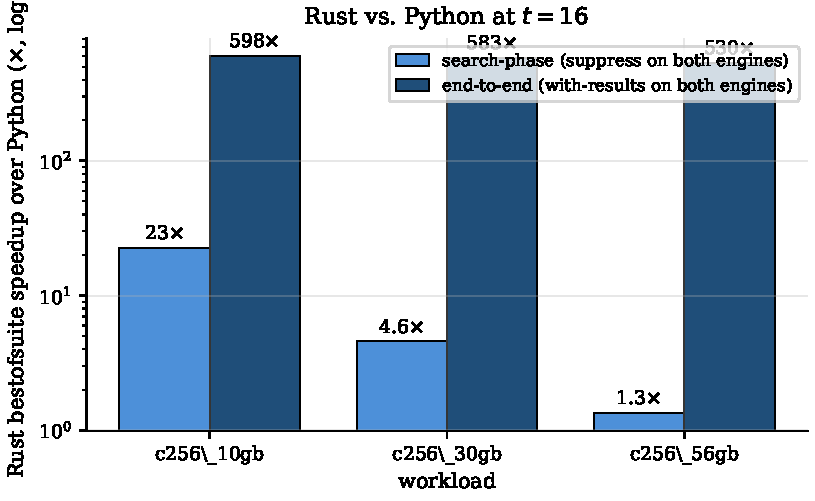
\includegraphics[width=0.9\linewidth]{img/gen/ch4_e2e_speedup.pdf}
  \caption{Rust \bcombo{} speedup over the Python baseline at $t=16$ across the three calibration workloads, End-to-end (with-results) stays in the $530$--$598\times$ range because of Python's per-\emph{(query, cluster)} result-dict construction. Search phase alone (suppress) drops monotonically from $22.7\times$ $\to$ $1.34\times$. Log $y$-axis.}
  \label{fig:exp:e2e_speedup}
\end{figure}

\section{Rust Rebinning Kernel\label{sec:exp:rebinning}}

We fuse the two stages of the Python rebinning (per-histogram rebinning under \texttt{multiprocessing.Pool}, then \texttt{numpy.cumsum} + \texttt{argsort(axis=0)} per cluster) into a single-threaded, in-place Rust call. Rust parallelizes the rebinning across all cores, followed by in-place cumsum and a stable \texttt{sort\_by}.

\begin{table}[H]
  \centering
  \caption{Rebinning kernel wall across the three calibration datasets, median of 3 reps.}
  \label{tab:rebin}
  \footnotesize
  \begin{tabular}{lrrr}
    \toprule
    Dataset & Python (\texttt{multiprocessing.Pool}) & Rust kernel & Speedup \\
    \midrule
    \texttt{c256\_10gb} ($324$\,K hists) & $83.5$\,s & $17.7$\,s & $4.72\times$ \\
    \texttt{c256\_30gb} ($997$\,K hists) & $306.5$\,s & $64.3$\,s & $4.77\times$ \\
    \texttt{c256\_56gb} ($5.02$\,M hists) & $3{,}220$\,s & $1{,}479$\,s & $2.18\times$ \\
    \bottomrule
  \end{tabular}
\end{table}

Correctness is verified against the Python reference on $200$ queries: the rounding-mode difference between Rust (round-half-away) and NumPy (banker's rounding) produces a maximum cumulative difference of $10^{-4}$ at a handful of histogram rows, which does not affect sort order or query results.

The kernel falls back to the Python pipeline if \texttt{fainder\_core} is not importable or if \texttt{bin\_estimation == \textquotesingle cubic\_spline\textquotesingle}.

\section{Variance Check on Borderline Claims\label{sec:exp:variance}}

Most claims in this chapter are far outside the noise floor, but a few are close enough to the noise floor that they were re-measured at $10$ reps per cell to tighten the interval, and one claim was re-verified against a variance probe.

\textbf{Fine-t f16 vs default on \texttt{c256\_56gb}} (§\ref{sec:exp:c2:f16}). Initially, under the $5$-rep sweep, the peak win was $\sim\!-10\%$ at $t{=}18$, but the $10$-rep upgrade brings the CI half-width from $\sim\!3.4\%$ to $\sim\!2.1\%$. Concluding that no cell shows a significant f16 standalone win.

\textbf{c1024 SIMD anomaly at $t{=}64$} (§\ref{sec:exp:ood:struct}). The $5$-rep sweep showed SIMD at $t{=}64$ measuring $-6.7\%$ vs baseline, an outlier to the $6/6$ null SIMD reproduction. The variance-probe run suggests the $t{=}64$ cell has anomalously high inter-run variance on this specific dataset.

\section{Summary\label{sec:exp:summary}}

Table~\ref{tab:exp:hyp_verdicts} revisits the a-priori hypotheses of §\ref{sec:method:hypotheses} against this chapter's evidence.

\begin{table}[H]
  \centering
  \caption{Hypotheses from Chapter~\ref{cha:chapter3} and their verdicts.}
  \label{tab:exp:hyp_verdicts}
  \footnotesize
  \begin{tabular}{>{\raggedright\arraybackslash}p{0.30\linewidth}>{\raggedright\arraybackslash}p{0.16\linewidth}>{\raggedright\arraybackslash}p{0.42\linewidth}}
    \toprule
    Hypothesis & Verdict & Evidence \\
    \midrule
    (i) Latency-side throughput reduces wall at every $t$ & Falsified & Four null ablations, $0.90$--$1.13\times$ across all cells (§\ref{sec:exp:c1}) \\
    (ii) Footprint reduction wins at intermediate $t$ & Refined & Binding constraint is regime-dependent: arena-mutex contention on the primary workload, L3-aggregate footprint at the OOD density; \texttt{f16} and \texttt{pooled} sign-flip inside the bundle (§\ref{sec:exp:c2}) \\
    (iii) Bandwidth reduction wins at high $t$ & Confirmed standalone; falsified in composition & \texttt{packed-ids} $-20\%$ standalone at high $t$; regresses over \bcombo{} in 12/18 cells (§\ref{sec:exp:c3}, §\ref{sec:exp:negcomp:instances}) \\
    (iv) NUMA probe separates on-socket pressure from UPI & Confirmed & Single-socket $-11$ to $-13\%$; interleave $+26$ to $+41\%$ (§\ref{sec:exp:c4}) \\
    Five predictions of positive composition & All falsified & Five instances on five hardware axes (§\ref{sec:exp:negcomp:instances}) \\
    Dispatch within $5\%$ in-distribution & Confirmed & $17/18$ exact, $18/18$ within $5\%$ (§\ref{sec:exp:dispatch}) \\
    OOD generalisation at the sparser density point & Confirmed & $6/6$ within $1\%$; $4$ strong $+$ $2$ clean reproductions, $2$ refinements, $0$ falsifications (§\ref{sec:exp:ood}) \\
    \bottomrule
  \end{tabular}
\end{table}

Four ceilings bind Fainder's percentile workload on this platform: single-thread compute / L1 latency (which never binds in practice), shared L3 capacity, on-socket memory-traffic pressure, and the cross-socket UPI interconnect. The latency-side optimisations (SIMD, batch-search, horizontal-SIMD, PGM) all measure null: they accelerate a stage that does not bind. The bandwidth-side optimisations (\texttt{f16}, \texttt{packed-ids}, \texttt{pooled}, \texttt{mimalloc}) and single-socket placement each move wall on their own ceiling.

These optimisations compose negatively. We show five instances on five hardware axes with respective \emph{perf} counters as evidence. It shows: the ceiling that binds at the composition is \emph{not} the one the second ablation attacks. This leads to the pre-flight methodology, where we probe the binding ceiling at the target composition before committing to an implementation.

The dispatch policy holds in-distribution ($17/18$ exact, $18/18$ within $5\%$) and out-of-distribution ($6/6$ within $5\%$ at $3.2\times$ sparser clusters). Ceilings (i) and (iv) reproduce across density while ceiling (ii) has a density-dependent threshold. Four of the five negative-composability instances reproduce in sign at the OOD point, and morsel scheduling attenuates to within-noise.

The Rust port that carried these measurements delivers $530$--$598\times$ end-to-end over the Python baseline at $t=16$, and $114\times$ at the only paired single-thread cell. Most of that ratio is Python's per-\emph{(query, cluster)} result materialisation ($96.9$--$99.8\%$ of its wall, §\ref{sec:exp:e2e:mat}). The search phase itself scales $22.7\times$, $4.6\times$, $1.34\times$ as per-cluster footprint grows into the shared ceilings. NUMA placement adds $11$--$13\%$ at $t \leq 48$, and the rebinning kernel a separate $\sim\!4.7\times$, dropping to $\sim\!2.2\times$ at five million histograms (§\ref{sec:exp:rebinning}).

What generalises beyond this codebase is the ceiling characterisation, the composition pattern, and the pre-flight methodology. The Rust port is the medium that produced them.